\documentclass[xcolor={dvipsnames}]{beamer}

\usepackage{enumerate}
\usepackage{MnSymbol,wasysym}

\usepackage[numbers]{natbib}

\def\labelenumii{\theenumi}

\setbeamertemplate{navigation symbols}{}

\newcommand{\cInjB}[1]{\mName{INJ2}(#1)}

%Information to be included in the title page:
\usetheme{Berlin}
\title{Alonzo in Alonzo}
\author{Christopher Schankula \& Dennis Yankovsky\\ (Group 1: ``See: Group Name'')}
\institute{CAS-760 Fall 2022, \\McMaster University}
\date{December 5th, 2022}

\renewcommand{\labelenumii}{\theenumii.}
\newcommand{\be}{\begin{enumerate}}
\newcommand{\ee}{\end{enumerate}}
\newcommand{\bi}{\begin{itemize}}
\newcommand{\ei}{\end{itemize}}
\newcommand{\bc}{\begin{center}}
\newcommand{\ec}{\end{center}}
\newcommand{\bsp}{\begin{sloppypar}}
\newcommand{\esp}{\end{sloppypar}}

\newcommand{\sA}{{\cal A}}
\newcommand{\sB}{{\cal B}}
\newcommand{\sC}{{\cal C}}
\newcommand{\sD}{{\cal D}}
\newcommand{\sE}{{\cal E}}
\newcommand{\sF}{{\cal F}}
\newcommand{\sG}{{\cal G}}
\newcommand{\sH}{{\cal H}}
\newcommand{\sI}{{\cal I}}
\newcommand{\sJ}{{\cal J}}
\newcommand{\sK}{{\cal K}}
\newcommand{\sL}{{\cal L}}
\newcommand{\sM}{{\cal M}}
\newcommand{\sN}{{\cal N}}
\newcommand{\sO}{{\cal O}}
\newcommand{\sP}{{\cal P}}
\newcommand{\sQ}{{\cal Q}}
\newcommand{\sR}{{\cal R}}
\newcommand{\sS}{{\cal S}}
\newcommand{\sT}{{\cal T}}
\newcommand{\sU}{{\cal U}}
\newcommand{\sV}{{\cal V}}
\newcommand{\sW}{{\cal W}}
\newcommand{\sX}{{\cal X}}
\newcommand{\sY}{{\cal Y}}
\newcommand{\sZ}{{\cal Z}}

\newcommand{\bA}{\mathbb{A}}
\newcommand{\bB}{\mathbb{B}}
\newcommand{\bC}{\mathbb{C}}
\newcommand{\bD}{\mathbb{D}}
\newcommand{\bE}{\mathbb{E}}
\newcommand{\bF}{\mathbb{F}}
\newcommand{\bG}{\mathbb{G}}
\newcommand{\bH}{\mathbb{H}}
\newcommand{\bI}{\mathbb{I}}
\newcommand{\bJ}{\mathbb{J}}
\newcommand{\bK}{\mathbb{K}}
\newcommand{\bL}{\mathbb{L}}
\newcommand{\bM}{\mathbb{M}}
\newcommand{\bN}{\mathbb{N}}
\newcommand{\bO}{\mathbb{O}}
\newcommand{\bP}{\mathbb{P}}
\newcommand{\bQ}{\mathbb{Q}}
\newcommand{\bR}{\mathbb{R}}
\newcommand{\bS}{\mathbb{S}}
\newcommand{\bT}{\mathbb{T}}
\newcommand{\bU}{\mathbb{U}}
\newcommand{\bV}{\mathbb{V}}
\newcommand{\bW}{\mathbb{W}}
\newcommand{\bX}{\mathbb{X}}
\newcommand{\bY}{\mathbb{Y}}
\newcommand{\bZ}{\mathbb{Z}}


\newcommand{\sglsp}{\ }
\newcommand{\dblsp}{\ \ }
\newcommand{\textrel}[1]{\dblsp \text{#1} \dblsp}

\newcommand{\TRUE}{\mbox{{\sc t}}}
\newcommand{\FALSE}{\mbox{{\sc f}}}
\newcommand{\Neg}{\neg} 
\ifdefined \And 
\renewcommand{\And}{\wedge}
\else
\newcommand{\And}{\wedge}
\fi
\newcommand{\Or}{\vee}
\newcommand{\Implies}{\Rightarrow}
\newcommand{\Iff}{\Leftrightarrow}
\newcommand{\Forall}{\forall}
\newcommand{\ForallApp}{\forall\,}
\newcommand{\Forsome}{\exists}
\newcommand{\ForsomeApp}{\exists\,}
\newcommand{\ForsomeUnique}{\exists!}
\newcommand{\ForsomeUniqueApp}{\exists!\,}
\newcommand{\LambdaApp}{\lambda\,}
\newcommand{\LAMBDAapp}{\Lambda\,}
\newcommand{\PiApp}{\Pi\,}
\newcommand{\SigmaApp}{\Sigma\,}
\newcommand{\iotaApp}{\iota\,}
\newcommand{\Iota}{{\rm I}}
\newcommand{\IotaApp}{{\rm I}\,}
\newcommand{\invertediota}{\rotatebox[origin=c]{180}{$\iota$}}
\newcommand{\epsilonApp}{\epsilon\,}
\newcommand{\Set}{\circledS}
\newcommand{\SetApp}{\circledS\,}

\newcommand{\IsDef}{\downarrow}
\newcommand{\IsUndef}{\uparrow}
\newcommand{\IsDefApp}{\,{\IsDef}}
\newcommand{\IsUndefApp}{\,{\IsUndef}}
\newcommand{\QuasiEqual}{\simeq}
\newcommand{\Undefined}{\bot}
\newcommand{\If}[3]{#1 \mapsto #2 \mid #3}
\newcommand{\SynEqual}{\equiv}

\renewcommand{\phi}{\varphi}
%\newcommand{\set}[1]{{\{#1\}}}
\newcommand{\seq}[1]{{\langle #1 \rangle}}
\newcommand{\seqlike}[1]{\seq{\!\seq{#1}\!}}
%\newcommand{\mlist}[1]{[#1]}
\newcommand{\compl}[1]{\overline{#1}}
\newcommand{\recip}[1]{{#1}^{-1}}
\newcommand{\pow}[1]{\sP(#1)}
\newcommand{\tarrow}{\rightarrow}
%\newcommand{\bo}{\omicron}
\newcommand{\consext}{\trianglelefteq}
\newcommand{\mIff}{\textrel{iff}}
\newcommand{\mImp}{\textrel{implies}}
\newcommand{\mEq}{\dblsp{=}\dblsp}
\newcommand{\mNotEq}{\dblsp{\not=}\dblsp}
\newcommand{\mQEq}{\dblsp{\simeq}\dblsp}
\newcommand{\mNotQEq}{\dblsp{\not\simeq}\dblsp}
\newcommand{\mIncluded}{\preceq}
\newcommand{\hr}{\phantom{}^\ast\mathbb{R}}
\newcommand{\restricted}{\mbox{$\upharpoonright$}\nolinebreak}
\newcommand{\subfun}{\sqsubseteq}
\newcommand{\clexpr}[1]{\overline{\sE_{#1}}}

\newcommand{\churchqe}{$\mbox{\sc ctt}_{\rm qe}$}
\newcommand{\churchuqe}{$\mbox{\sc ctt}_{\rm uqe}$}
\newcommand{\qzero}{${\cal Q}_0$}
\newcommand{\qzerou}{${\cal Q}^{\rm u}_{0}$}
\newcommand{\qzerouqe}{${\cal Q}^{\rm uqe}_{0}$}
\newcommand{\fstar}{${\rm F}^\ast$}

\newenvironment{proof}[1][\unskip]{\par\noindent{\bf Proof{#1}\dblsp}}{\hfill$\Box$}

\newcommand{\urlpart}[1]{\mbox{\texttt{#1}}\linebreak[0]}

%% LaTeX Macros for Alonzo Notation
%%
%% William M. Farmer
%%
%% McMaster University

%% Requires:

\usepackage{amssymb}
\usepackage{amsmath}
\usepackage{phonetic}
\usepackage[dvipsnames]{xcolor}

%%%%%%%%%%%%%%%%%%%%%%%%%%%%%%%%%%%%%%%%%%%%%%%%%%%%%%%%%%%%%%%%%

% MISCELLANEOUS MACROS

\newcommand{\mName}[1]{\mathsf{#1}}
\newcommand{\mSet}[1]{\{ #1 \}}
\newcommand{\mTuple}[1]{( #1 )}
\newcommand{\mList}[1]{[ #1 ]}
\newcommand{\mSeq}[1]{\langle #1 \rangle}
\newcommand{\mSeqlike}[1]{\mSeq{\!\mSeq{#1}\!}}
\newcommand{\mAbs}[1]{\lvert #1 \rvert}
\newcommand{\mNorm}[1]{\lVert #1 \rVert}
\newcommand{\mDot}{\mathrel{.}}

%%%%%%%%%%%%%%%%%%%%%%%%%%%%%%%%%%%%%%%%%%%%%%%%%%%%%%%%%%%%%%%%%

% FORMAL NOTATION

% Types

\newcommand{\fBoolTy}{\mName{BoolTy}}
\newcommand{\fBaseTy}[1]{\mName{BaseTy}(#1)}
\newcommand{\fFunTy}[2]{\mName{FunTy}(#1,#2)}
\newcommand{\fProdTy}[2]{\mName{ProdTy}(#1,#2)}

% Expressions

\newcommand{\fVar}[2]{\mName{Var}(#1,#2)}
\newcommand{\fCon}[2]{\mName{Con}(#1,#2)}
\newcommand{\fEq}[2]{\mName{Eq}(#1,#2)}
\newcommand{\fFunApp}[2]{\mName{FunApp}(#1,#2)}
\newcommand{\fFunAbs}[3]{\mName{FunAbs}(\fVar{#1}{#2},#3)}
\newcommand{\fDefDes}[3]{\mName{DefDes}(\fVar{#1}{#2},#3)}
\newcommand{\fOrdPair}[2]{\mName{OrdPair}(#1,#2)}

%%%%%%%%%%%%%%%%%%%%%%%%%%%%%%%%%%%%%%%%%%%%%%%%%%%%%%%%%%%%%%%%%

% COMPACT NOTATION

% Types

\newcommand{\cBoolTy}{\omicron}
\newcommand{\cB}{\cBoolTy}
\newcommand{\cBaseTy}[1]{#1}
\newcommand{\cFunTy}[2]{({#1} \rightarrow {#2})}
\newcommand{\cFunTyX}[2]{{#1} \rightarrow {#2}}
\newcommand{\cFunTyB}[3]{\cFunTy {#1} {\cFunTyX {#2} {#3}}}
\newcommand{\cFunTyBX}[3]{\cFunTyX {#1} {\cFunTyX {#2} {#3}}}
\newcommand{\cFunTyC}[4]{\cFunTy {#1} {\cFunTyX {#2} {\cFunTyX {#3} {#4}}}}
\newcommand{\cFunTyCX}[4]{\cFunTyX {#1} {\cFunTyX {#2} {\cFunTyX {#3} {#4}}}}
\newcommand{\cProdTy}[2]{({#1} \times {#2})}
\newcommand{\cProdTyX}[2]{{#1} \times {#2}}
\newcommand{\cProdTyB}[3]{\cProdTy {#1} {\cProdTyX {#2} {#3}}}
\newcommand{\cProdTyBX}[3]{\cProdTyX {#1} {\cProdTyX {#2} {#3}}}
\newcommand{\cProdTyC}[4]{\cProdTy {#1} {\cProdTyX {#2} {\cProdTyX {#3} {#4}}}}
\newcommand{\cProdTyCX}[4]{\cProdTyX {#1} {\cProdTyX {#2} {\cProdTyX {#3} {#4}}}}

% Expressions

\newcommand{\cVar}[2]{({#1} : {#2})}
\newcommand{\cVarY}[2]{#1}
\newcommand{\cCon}[2]{{#1}_{#2}}
\newcommand{\cConY}[2]{#1}
\newcommand{\cEq}[2]{({#1} = {#2})}
\newcommand{\cEqX}[2]{{#1} = {#2}}
\newcommand{\cFunApp}[2]{(#1\,#2)}
\newcommand{\cFunAppX}[2]{#1\,#2}
\newcommand{\cFunAppB}[3]{(\cFunAppX {\cFunAppX {#1} {#2}} {#3})}
\newcommand{\cFunAppBX}[3]{\cFunAppX {\cFunAppX {#1} {#2}} {#3}}
\newcommand{\cFunAppC}[4]{(\cFunAppX {\cFunAppX {\cFunAppX {#1}{#2}}{#3}}{#4})}
\newcommand{\cFunAppCX}[4]{\cFunAppX {\cFunAppX {\cFunAppX {#1}{#2}}{#3}}{#4}}
\newcommand{\cFunAbs}[3]{(\lambda\, #1 : #2 \mDot #3)}
\newcommand{\cFunAbsX}[3]{\lambda\, #1 : #2 \mDot #3}
\newcommand{\cDefDes}[3]{(\mathrm{I}\, #1 : #2 \mDot #3)}
\newcommand{\cDefDesX}[3]{\mathrm{I}\, #1 : #2 \mDot #3}
\newcommand{\cOrdPair}[2]{(#1,#2)}

% Boolean Operators

\newcommand{\cTPC}{T_\cB}
\newcommand{\cT}{\cTPC}
\newcommand{\cFPC}{F_\cB}
\newcommand{\cF}{\cFPC}
\newcommand{\cAndPC}{\wedge_{\cFunTyBX{\cB}{\cB}{\cB}}}
\newcommand{\cAnd}[2]{({#1} \wedge {#2})}
\newcommand{\cAndX}[2]{{#1} \wedge {#2}}
\newcommand{\cAndB}[3]{\cAnd {#1} {\cAndX {#2} {#3}}}
\newcommand{\cAndBX}[3]{\cAndX {#1} {\cAndX {#2} {#3}}}
\newcommand{\cAndL}[1]{(#1)}   % separator is $\And$
\newcommand{\cAndLX}[1]{#1}    % separator is $\And$
\newcommand{\cImpliesPC}{\Rightarrow_{\cFunTyBX {\cB} {\cB} {\cB}}}
\newcommand{\cImplies}[2]{({#1} \Rightarrow {#2})}
\newcommand{\cImpliesX}[2]{{#1} \Rightarrow {#2}}
\newcommand{\cNegPC}{\neg_{\cFunTyX{\cB}{\cB}}}
\newcommand{\cNeg}[1]{(\neg{#1})}
\newcommand{\cNegX}[1]{\neg{#1}}
\newcommand{\cOrPC}{\vee_{\cFunTyBX{\cB}{\cB}{\cB}}}
\newcommand{\cOr}[2]{({#1} \vee {#2})}
\newcommand{\cOrX}[2]{{#1} \vee {#2}}
\newcommand{\cOrB}[3]{\cOr {#1} {\cOrX {#2} {#3}}}
\newcommand{\cOrBX}[3]{\cOrX {#1} {\cOrX {#2} {#3}}}
\newcommand{\cOrL}[1]{(#1)}    % separator is $\Or$
\newcommand{\cOrLX}[1]{#1}     % separator is $\Or$
\newcommand{\cIfPC}[1]{\mName{if}_{\cFunTyCX{\cB}{#1}{#1}{#1}}}
\newcommand{\cIf}[3]{(#1 \mapsto #2 \mid #3)}
\newcommand{\cIfX}[3]{#1 \mapsto #2 \mid #3}

% Binary Operators

\newcommand{\cBin}[3]{({#1} \mathrel{#2} {#3})}
\newcommand{\cBinX}[3]{{#1} \mathrel{#2} {#3}}
\newcommand{\cBinB}[5]{({#1} \mathrel{#2} {#3} \mathrel{#4} {#5})}
\newcommand{\cBinBX}[5]{{#1} \mathrel{#2} {#3} \mathrel{#4} {#5}}
\newcommand{\cIff}[2]{({#1} \Leftrightarrow {#2})}
\newcommand{\cIffX}[2]{{#1} \Leftrightarrow {#2}}
\newcommand{\cNotEq}[2]{({#1} \not= {#2})}
\newcommand{\cNotEqX}[2]{{#1} \not= {#2}}

% Quantifiers

\newcommand{\cForall}[3]{(\forall\, #1 : #2 \mDot #3)}
\newcommand{\cForallX}[3]{\forall\, #1 : #2 \mDot #3}
\newcommand{\cForallB}[5]{(\forall\, #1 : #2,\, #3 : #4 \mDot #5)}
\newcommand{\cForallBX}[5]{\forall\, #1 : #2,\, #3 : #4 \mDot #5}
\newcommand{\cForallC}[7]{(\forall\, #1 : #2,\, #3 : #4,\, #5 : #6 \mDot #7)}
\newcommand{\cForallCX}[7]{\forall\, #1 : #2,\, #3 : #4,\, #5 : #6 \mDot #7}
\newcommand{\cForsome}[3]{(\exists\, #1 : #2 \mDot #3)}
\newcommand{\cForsomeX}[3]{\exists\, #1 : #2 \mDot #3}
\newcommand{\cForsomeB}[5]{(\exists\, #1 : #2,\, #3 : #4 \mDot #5)}
\newcommand{\cForsomeBX}[5]{\exists\, #1 : #2,\, #3 : #4 \mDot #5}
\newcommand{\cForsomeC}[7]{(\exists\, #1 : #2,\, #3 : #4,\, #5 : #6 \mDot #7)}
\newcommand{\cForsomeCX}[7]{\exists\, #1 : #2,\, #3 : #4,\, #5 : #6 \mDot #7}
\newcommand{\cForsomeUnique}[3]{(\exists!\, #1 : #2 \mDot #3)}
\newcommand{\cForsomeUniqueX}[3]{\exists!\, #1 : #2 \mDot #3}
\newcommand{\cForsomeUniqueB}[5]{(\exists!\, #1 : #2, \, #3 : #4 \mDot #5)}
\newcommand{\cForsomeUniqueBX}[5]{\exists!\, #1 : #2, \, #3 : #4 \mDot #5}
\newcommand{\cForsomeUniqueC}[7]{(\exists!\, #1 : #2, \, #3 : #4, \, #5 : #6     \mDot #7)}
\newcommand{\cForsomeUniqueCX}[7]{\exists!\, #1 : #2, \, #3 : #4, \, #5 : #6     \mDot #7}
% Definedness

\newcommand{\cBotPC}[1]{\bot_{#1}}
\newcommand{\cEmpFunPC}[2]{\Delta_{\cFunTyX {#1} {#2}}}
\newcommand{\cIsDef}[1]{(#1{\downarrow})}
\newcommand{\cIsDefX}[1]{#1{\downarrow}}
\newcommand{\cIsUndef}[1]{(#1{\uparrow})}
\newcommand{\cIsUndefX}[1]{#1{\uparrow}}
\newcommand{\cQuasiEq}[2]{({#1} \simeq {#2})}
\newcommand{\cQuasiEqX}[2]{{#1} \simeq {#2}}
\newcommand{\cNotQuasiEq}[2]{({#1} \not\simeq {#2})}
\newcommand{\cNotQuasiEqX}[2]{{#1} \not\simeq {#2}}

% Sets

\newcommand{\cSetTy}[1]{\mSet{#1}}
\newcommand{\cIn}[2]{({#1} \in {#2})}
\newcommand{\cInX}[2]{{#1} \in {#2}}
\newcommand{\cNotIn}[2]{({#1} \not\in {#2})}
\newcommand{\cNotInX}[2]{{#1} \not\in {#2}}
\newcommand{\cSet}[3]{\mSet{{{#1} : {#2}} \mid {#3}}}
\newcommand{\cEmpSetPC}[1]{\emptyset_{\cSetTy {#1}}}
\newcommand{\cEmpSetAltPC}[1]{\mSet{\,}_{\cSetTy {#1}}}
\newcommand{\cUnivSetPC}[1]{U_{\cSetTy {#1}}}
\newcommand{\cFinSet}[2]{\textsf{{$#1$}-{$#2$}-SET}}
\newcommand{\cFinSetL}[1]{\mSet{#1}}  % separator is ","
\newcommand{\cSubseteqPC}[1]{\subseteq_{\cFunTyBX {\cSetTy #1} {\cSetTy #1} {\cB}}}
\newcommand{\cUnionPC}[1]{\cup_{\cFunTyBX {\cSetTy #1} {\cSetTy #1} {\cSetTy #1}}}
\newcommand{\cUnion}[2]{\cBin {#1} {\cup} {#2}}
\newcommand{\cUnionX}[2]{\cBinX {#1} {\cup} {#2}}
\newcommand{\cIntersPC}[1]{\cap_{\cFunTyBX {\cSetTy #1} {\cSetTy #1} {\cSetTy #1}}}
\newcommand{\cInters}[2]{\cBin {#1} {\cap} {#2}}
\newcommand{\cIntersX}[2]{\cBinX {#1} {\cap} {#2}}
\newcommand{\cComplPC}[1]{\overline{\,\cdot\,}_{\cFunTyX {\cSetTy #1} {\cSetTy #1}}}
\newcommand{\cCompl}[1]{\overline{#1}}

% Tuples

\newcommand{\cTupleTyL}[1]{(#1)}  % separator is $\times$
\newcommand{\cTupleL}[1]{(#1)}    % separator is ","
\newcommand{\cFstPC}[2]{\mName{fst}_{\cFunTyX {\cProdTy {#1} {#2}} {#1}}}
\newcommand{\cSndPC}[2]{\mName{snd}_{\cFunTyX {\cProdTy {#1} {#2}} {#2}}}

% Functions

\newcommand{\cDomPC}[2]{\mName{dom}_{\cFunTyX {\cFunTy {#1} {#2}} {\cSetTy {#1}}}}
\newcommand{\cRanPC}[2]{\mName{ran}_{\cFunTyX {\cFunTy {#1} {#2}} {\cSetTy {#2}}}}
\newcommand{\cSubfuneqPC}[2]{\subfun_{\cFunTyBX {\cFunTy {#1} {#2}} {\cFunTy {#1} {#2}} {\cB}}}
\newcommand{\cFunCompPC}[3]{\circ_{\cFunTyBX {\cFunTy {#1} {#2}} {\cFunTy {#2} {#3}} {\cFunTy {#1} {#3}}}}
\newcommand{\cFunComp}[2]{({#1} \circ {#2})}
\newcommand{\cFunCompX}[2]{#1 \circ {#2}}
\newcommand{\cRestrictPC}[2]{\restricted_{\cFunTyBX {\cFunTy {#1} {#2}} {\cSetTy {#1}} {\cFunTy {#1} {#2}}}}
\newcommand{\cRestrict}[2]{(#1 \restricted_{#2})}
\newcommand{\cRestrictX}[2]{#1 \restricted_{#2}}

% Miscellaneous Notation

\newcommand{\cTotal}[1]{\mName{TOTAL}(#1)}
\newcommand{\cTotalB}[1]{\mName{TOTAL2}(#1)}
\newcommand{\cSurj}[1]{\mName{SURJ}(#1)}
\newcommand{\cSurjB}[1]{\mName{SURJ2}(#1)}
\newcommand{\cInj}[1]{\mName{INJ}(#1)}
\newcommand{\cBij}[1]{\mName{BIJ}(#1)}
\newcommand{\cDistinctL}[1]{\mName{DISTINCT}(#1)}  % separator is ","

% Quasitypes

\newcommand{\cFunAbsQTy}[3]{\cFunAbs {#1} {#2} {#3}}
\newcommand{\cFunAbsQTyX}[3]{\cFunAbsX {#1} {#2} {#3}}
\newcommand{\cForallQTy}[3]{\cForall {#1} {#2} {#3}}
\newcommand{\cForallQTyX}[3]{\cForallX {#1} {#2} {#3}}
\newcommand{\cForallQTyB}[5]{\cForallB {#1} {#2} {#3} {#4} {#5}}
\newcommand{\cForallQTyBX}[5]{\cForallBX {#1} {#2} {#3} {#4} {#5}}
\newcommand{\cForsomeQTy}[3]{\cForsome {#1} {#2} {#3}}
\newcommand{\cForsomeQTyX}[3]{\cForsomeX {#1} {#2} {#3}}
\newcommand{\cForsomeQTyB}[5]{\cForsomeB {#1} {#2} {#3} {#4} {#5}}
\newcommand{\cForsomeQTyBX}[5]{\cForsomeBX {#1} {#2} {#3} {#4} {#5}}
\newcommand{\cDefDesQTy}[3]{\cDefDes {#1} {#2} {#3}}
\newcommand{\cDefDesQTyX}[3]{\cDefDesX {#1} {#2} {#3}}
\newcommand{\cIsDefInQTy}[2]{({#1} \downarrow {#2})}
\newcommand{\cIsDefInQTyX}[2]{{#1} \downarrow {#2}}
\newcommand{\cIsUndefInQTy}[2]{({#1} \uparrow {#2})}
\newcommand{\cIsUndefInQTyX}[2]{{#1} \uparrow {#2}}
\newcommand{\cFunQTyPC}[2]{\rightarrow_{\cFunTyBX {\cSetTy {#1}} {\cSetTy {#2}} {\cSetTy {\cFunTyX {#1} {#2}}}}}
\newcommand{\cFunQTy}[2]{\cFunTy {#1} {#2}}
\newcommand{\cFunQTyX}[2]{\cFunTyX {#1} {#2}}
\newcommand{\cFunQTyB}[3]{\cFunTyB {#1} {#2} {#3}}
\newcommand{\cFunQTyBX}[3]{\cFunTyBX {#1} {#2} {#3}}
\newcommand{\cFunQTyC}[4]{\cFunTyC {#1} {#2} {#3} {#4}}
\newcommand{\cFunQTyCX}[4]{\cFunTyCX {#1} {#2} {#3} {#4}}
\newcommand{\cProdQTyPC}[2]{\times_{\cFunTyBX {\cSetTy {#1}} {\cSetTy {#2}} {\cSetTy {\cProdTyX {#1} {#2}}}}}
\newcommand{\cProdQTy}[2]{\cProdTy {#1} {#2}}
\newcommand{\cProdQTyX}[2]{\cProdTyX {#1} {#2}}
\newcommand{\cProdQTyB}[3]{\cProdTyB {#1} {#2} {#3}}
\newcommand{\cProdQTyBX}[3]{\cProdTyBX {#1} {#2} {#3}}
\newcommand{\cProdQTyC}[4]{\cProdTyC {#1} {#2} {#3} {#4}}
\newcommand{\cProdQTyCX}[4]{\cProdTyCX {#1} {#2} {#3} {#4}}
\newcommand{\cTotalOn}[3]{\textsf{TOTAL-ON}(#1,#2,#3)}
\newcommand{\cTotalOnB}[4]{\textsf{TOTAL-ON2}(#1,#2,#3,#4)}
\newcommand{\cSurjOn}[3]{\textsf{SURJ-ON}(#1,#2,#3)}
\newcommand{\cSurjOnB}[4]{\textsf{SURJ-ON2}(#1,#2,#3,#4)}
\newcommand{\cInjOn}[2]{\textsf{INJ-ON}(#1,#2)}
\newcommand{\cBijOn}[3]{\textsf{BIJ-ON}(#1,#2,#3)}
\newcommand{\cInf}[1]{\mName{INF}(#1)}
\newcommand{\cFin}[1]{\mName{FIN}(#1)}
\newcommand{\cCount}[1]{\mName{COUNT}(#1)}

% Dependent Quasitypes

\newcommand{\cPiTy}[2]{\cFunTyBX {\cSetTy {#1}} {\cFunTy {#1} {\cSetTy {#2}}} {\cSetTy {\cFunTyX {#1} {#2}}}}
\newcommand{\cPiPC}[2]{\Pi_{\cPiTy {#1} {#2}}}
\newcommand{\cPi}[3]{(\Pi\, #1 : #2 \mDot #3)}
\newcommand{\cPiX}[3]{\Pi\, #1 : #2 \mDot #3}
\newcommand{\cSigmaTy}[2]{\cFunTyBX {\cSetTy {#1}} {\cFunTy {#1} {\cSetTy {#2}}} {\cSetTy {\cProdTyX {#1} {#2}}}}
\newcommand{\cSigmaPC}[2]{\Sigma_{\cSigmaTy {#1} {#2}}}
\newcommand{\cSigma}[3]{(\Sigma\, #1 : #2 \mDot #3)}
\newcommand{\cSigmaX}[3]{\Sigma\, #1 : #2 \mDot #3}

% Sequences

\newcommand{\cSequencesPC}[2]{\mName{sequences}_{\cSetTy {\cFunTyX {#1} {#2}}}}
\newcommand{\cSeqQTy}[1]{\mSeqlike{#1}}
\newcommand{\cStreamsPC}[2]{\mName{streams}_{\cSetTy {\cFunTyX {#1} {#2}}}}
\newcommand{\cSeqInfQTy}[1]{\mSeq{#1}}
\newcommand{\cListsPC}[2]{\mName{lists}_{\cSetTy {\cFunTyX {#1} {#2}}}}
\newcommand{\cSeqFinQTy}[1]{\mList{#1}}
\newcommand{\cConsPC}[2]{\mName{cons}_{\cFunTyBX {#2} {\cFunTy {#1} {#2}} {\cFunTy {#1} {#2}}}}
\newcommand{\cCons}[2]{({#1} :: {#2})}
\newcommand{\cConsX}[2]{{#1} :: {#2}}
\newcommand{\cHdPC}[2]{\mName{hd}_{\cFunTyX {\cFunTy {#1} {#2}} {#2}}}
\newcommand{\cTlPC}[2]{\mName{tl}_{\cFunTyX {\cFunTy {#1} {#2}} {\cFunTy {#1} {#2}}}}
\newcommand{\cNilPC}[2]{\mName{nil}_{\cFunTyX {#1} {#2}}}
\newcommand{\cEmpListPC}[2]{{\mList{\;}}_{\cFunTyX {#1} {#2}}}
\newcommand{\cListL}[1]{\mList{#1}}  % separator is ","
\newcommand{\cLenPC}[2]{\mName{len}_{\cFunTyX {\cFunTy {#1} {#2}} {#1}}}
\newcommand{\cLen}{\mAbs}
\newcommand{\cNlistsPC}[2]{\mName{nlists}_{\cFunTyX {#1} {\cSetTy {\cFunTyX {#1} {#2}}}}}
\newcommand{\cSeqNFinQTy}[2]{\mList{#1}^{#2}}

% Real Numbers

\newcommand{\cRecip}{\recip}
\newcommand{\cFrac}{\frac}
\newcommand{\cAbs}{\mAbs}
\newcommand{\cSqrt}{\sqrt}
\newcommand{\cNorm}{\mNorm}
\newcommand{\cSum}[4]{\sum\limits_{{#1} = {#2}}^{#3} {#4}}
\newcommand{\cProd}[4]{\prod\limits_{{#1} = {#2}}^{#3} {#4}}
\newcommand{\cLim}[3]{\lim\limits_{{#1} \to {#2}} {#3}}
\newcommand{\cRightLim}[3]{\lim\limits_{{#1} \to {#2}^+} {#3}}
\newcommand{\cLeftLim}[3]{\lim\limits_{{#1} \to {#2}^-} {#3}}
\newcommand{\cLimSeq}[2]{\lim\limits_{{#1} \to \infty} {#2}}
\newcommand{\cIntegral}[4]{\int_{#1}^{#2} {#3}\,d{#4}}

%%%%%%%%%%%%%%%%%%%%%%%%%%%%%%%%%%%%%%%%%%%%%%%%%%%%%%%%%%%%%%%%%

% THEOREM ENVIRONMENTS

\newtheorem{thm}{Theorem}[section]
\newtheorem{cor}[thm]{Corollary}
\newtheorem{lem}[thm]{Lemma}
\newtheorem{prop}[thm]{Proposition}
\newtheorem{eg}[thm]{Example}
\newtheorem{rem}[thm]{Remark}

\newtheorem{thydef}[thm]{Theory Definition}
\newtheorem{thyext}[thm]{Theory Extension}
\newtheorem{devdef}[thm]{Development Definition}
\newtheorem{devext}[thm]{Development Extension}
\newtheorem{thytransdef}[thm]{Theory Translation Definition}
\newtheorem{thytransext}[thm]{Theory Translation Extension}
\newtheorem{devtransdef}[thm]{Development Translation Definition}
\newtheorem{devtransext}[thm]{Development Translation Extension}
\newtheorem{deftransport}[thm]{Definition Transportation}
\newtheorem{thmtransport}[thm]{Theorem Transportation}

%%%%%%%%%%%%%%%%%%%%%%%%%%%%%%%%%%%%%%%%%%%%%%%%%%%%%%%%%%%%%%%%%

% ENVIRONMENTS

\newenvironment{theory-def}[6]
{
\color{brown}
\begin{thydef}[#1]\em
\noindent
\begin{itemize} \setlength{\itemsep}{0pt}
\item[]\hspace{-3ex}\textbf{Name:} #2
\item[]\hspace{-3ex}\textbf{Base types:} #3
\item[]\hspace{-3ex}\textbf{Constants:} #4
\item[]\hspace{-3ex}\textbf{Axioms:} #5
\end{itemize}
 #6
\end{thydef} 
}

\newenvironment{theory-ext}[7]
{
\color{brown}
\begin{thyext}[#1]\em
\noindent
\begin{itemize} \setlength{\itemsep}{0pt}
\item[]\hspace{-3ex}\textbf{Name:} #2
\item[]\hspace{-3ex}\textbf{Extends\ } #3
\item[]\hspace{-3ex}\textbf{New base types:} #4
\item[]\hspace{-3ex}\textbf{New constants:} #5
\item[]\hspace{-3ex}\textbf{New axioms:} #6
\end{itemize}
#7
\end{thyext}
}

\newenvironment{dev-def}[4]
{
\color{brown}
\begin{devdef}[#1]\em
\noindent
\begin{itemize}
\item[]\hspace{-3ex}\textbf{Name:} #2
\item[]\hspace{-3ex}\textbf{Bottom theory:} #3
\item[]\hspace{-3ex}\textbf{Definitions and theorems:}
\end{itemize}
#4
\end{devdef}
}

\newenvironment{dev-ext}[4]
{
\color{brown}
\begin{devext}[#1]\em
\noindent
\begin{itemize}
\item[]\hspace{-3ex}\textbf{Name:} #2
\item[]\hspace{-3ex}\textbf{Extends\ } #3
\item[]\hspace{-3ex}\textbf{New definitions and theorems:}
\end{itemize}
#4
\end{devext}
}

\newenvironment{theory-trans-def}[6]
{
\color{brown}
\begin{thytransdef}[#1]\em
\noindent
\begin{itemize}
\item[]\hspace{-3ex}\textbf{Name:} #2
\item[]\hspace{-3ex}\textbf{Source theory:} #3
\item[]\hspace{-3ex}\textbf{Target theory:} #4
\item[]\hspace{-3ex}\textbf{Base type mapping:}
\end{itemize}
#5
\begin{itemize}
\item[]\hspace{-3ex}\textbf{Constant mapping:}
\end{itemize}
#6
\end{thytransdef}
}

\newenvironment{theory-trans-ext}[7]
{
\color{brown}
\begin{thytransext}[#1]\em
\noindent
\begin{itemize}
\item[]\hspace{-3ex}\textbf{Name:} #2
\item[]\hspace{-3ex}\textbf{Extends\ } #3
\item[]\hspace{-3ex}\textbf{New source theory:} #4
\item[]\hspace{-3ex}\textbf{New target theory:} #5
\item[]\hspace{-3ex}\textbf{New base type mapping:}
\end{itemize}
#6
\begin{itemize}
\item[]\hspace{-3ex}\textbf{New constant mapping:}
\end{itemize}
#7
\end{thytransext}
}

\newenvironment{dev-trans-def}[6]
{
\color{brown}
\begin{devtransdef}[#1]\em
\noindent
\begin{itemize}
\item[]\hspace{-3ex}\textbf{Name:} #2
\item[]\hspace{-3ex}\textbf{Source development:} #3
\item[]\hspace{-3ex}\textbf{Target development:} #4
\item[]\hspace{-3ex}\textbf{Base type mapping:}
\end{itemize}
#5
\begin{itemize}
\item[]\hspace{-3ex}\textbf{Constant mapping:}
\end{itemize}
#6
\end{devtransdef}
}

\newenvironment{dev-trans-ext}[6]
{
\color{brown}
\begin{devtransext}[#1]\em
\noindent
\begin{itemize}
\item[]\hspace{-3ex}\textbf{Name:} #2
\item[]\hspace{-3ex}\textbf{Extends\ } #3
\item[]\hspace{-3ex}\textbf{New source development:} #4
\item[]\hspace{-3ex}\textbf{New target development:} #5
\end{itemize}
\begin{itemize}
\item[]\hspace{-3ex}\textbf{New defined constant mapping:}
\end{itemize}
#6
\end{devtransext}
}

\newenvironment{def-transport}[7]
{
\color{brown}
\begin{deftransport}[#1]\em
\noindent
\begin{itemize}
\item[]\hspace{-3ex}\textbf{Name:} #2
\item[]\hspace{-3ex}\textbf{Development morphism:} #3
\item[]\hspace{-3ex}\textbf{Definition:}
\end{itemize}
#4
\begin{itemize}
\item[]\hspace{-3ex}\textbf{Transported definition:}
\end{itemize}
#5
\begin{itemize}
\item[]\hspace{-3ex}\textbf{New target development:} #6
\item[]\hspace{-3ex}\textbf{New development translation:} #7
\end{itemize}
\end{deftransport}
}

\newenvironment{thm-transport}[6]
{
\color{brown}
\begin{thmtransport}[#1]\em
\noindent
\begin{itemize}
\item[]\hspace{-3ex}\textbf{Name:} #2
\item[]\hspace{-3ex}\textbf{Development morphism:} #3
\item[]\hspace{-3ex}\textbf{Theorem:}
\end{itemize}
#4
\begin{itemize}
\item[]\hspace{-3ex}\textbf{Transported theorem:}
\end{itemize}
#5
\begin{itemize}
\item[]\hspace{-3ex}\textbf{New target development:} #6
\end{itemize}
\end{thmtransport}
}



\begin{document}

\newcommand\boxednumber[1]
{%
  \hbox{%
    \usebeamerfont*{item projected}%
    \usebeamercolor[bg]{item projected}%
    \vrule width2.25ex height1.85ex depth.4ex%
    \hskip-2.25ex%
    \hbox to2.25ex{%
      \hfil%
      \color{fg}#1%
      \hfil}%
  }%
}

\newcommand*{\squareref}[1]{
  \hbox{%
    \usebeamerfont*{item projected}%
    \usebeamercolor[bg]{item projected}%
    \vrule width2.25ex height1.85ex depth.4ex%
    \hskip-2.25ex%
    \hbox to2.25ex{%
      \hfil%
      \color{fg}\ref{#1}%
      \hfil}%
  }%
}

\frame{\titlepage}

\title{Alo\color{lightgray}alonzo\color{white}nzo}
\frame{\titlepage}

\author{Christopher Schankula \& Dennis Yankovsky}

\section{Introduction}
\begin{frame}
\frametitle{Scope}
\begin{itemize}
\item The scope for the project was to encode Alonzo types, expressions, free and bound variables, and 
substitutions in Alonzo
\item Stretch goals include encoding theories and semantics
\item For brevity, this presentation will focus only on types, pre-expressions and expressions
\end{itemize}
\end{frame}

% \begin{frame}
% \frametitle{Goals}
% \begin{itemize}
% \item Use Alonzo to describe and formalize Alonzo syntax
% \item Allow users to write expressions in a type-safe way
% \item Encode Alonzo syntax rules in such a way that syntax errors are impossible
% \item Gain a deeper understanding of Alonzo's type system and how expressions and types are constructed
% \end{itemize}
% \end{frame}

\begin{frame}
\frametitle{Conventions: The first major problem!}
\begin{itemize}
\item As we started talking about the project, within 5 minutes we realized we were getting ourselves confused really easily!
\item For example, does the word ``type'' refer to an actual Alonzo type, or a type in our new ``Alonzo''?
\item Thus, we settled on some conventions we will use throughout the presentation:
    \begin{itemize}
    \item ``Outer Alonzo'' refers to the ``real'' Alonzo we all know and love
    \item ``Inner Alonzo'' or ``Alo'' refers to our encoding of Alonzo inside Alonzo
    \item ``Alo'' type constructors all have the suffix ``AloTy'' to differentiate them from outer Alonzo's type constructors
    \item Similarly, ``Alo'' expression constructors all have the suffix ``Expr''
    \end{itemize}
\end{itemize}
\end{frame}

\begin{frame}
\frametitle{``But wait! Alonzo inside Alonzo? Is that even possible?''}
\begin{itemize}
\item Nope \cite{smullyan1992godel}. Not entirely, anyway.
\item<only@2> Tarski's theorem of the undefinability of truth; sufficiently strong systems cannot formalize their own semantics
\item<only@2> G\"{o}del's second incompleteness theorem; proving consistency
\end{itemize}
\end{frame}

\begin{frame}
\frametitle{Two different approaches}
\begin{itemize}
\item In our early discussions with Bill, we identified two different approaches we could take:
    \begin{enumerate}
        \item Alonzo expressions as strings of characters
        \item Alonzo expressions as an abstract syntax tree
    \end{enumerate}
\item We decided to take approach \#2 as it more closely matches Alonzo's definition, and it is easier to
reason about
\end{itemize}
\end{frame}

\section{Strings}
\begin{frame}
\frametitle{Strings}
\begin{thydef}[Strings]
\noindent
\begin{itemize} \setlength{\itemsep}{0pt}\vspace{-0.5cm}
\item<only@1>[]\hspace{-3ex}\textbf{Name:} $\mName{STR}$
\item<only@1>[]\hspace{-3ex}\textbf{Base types:} $C, S$
\item<only@1>[]\hspace{-3ex}\textbf{Constants:}\newline
{$\text{Stringify}_{\cFunTyX{\cBaseTy{C}}{\cBaseTy{S}}}$, $\text{Append}_{\cFunTyBX{\cBaseTy{C}}{\cBaseTy{S}}{\cBaseTy{S}}}$,
$A_C, B_C, C_C, ... , Z_C$.}
\item<only@2>[]\hspace{-3ex}\textbf{Axioms:}
{\be
\item $\cDistinctL{A,B,C,...,Z}$
\item $\forall c_1, c_2: \text{C}, s: S\ .\ \text{Stringify } c_1 \neq \text{Append } c_2\ s$
\item $\cInj{\text{Stringify}}$
\item $\cTotal{\text{Stringify}}$
\item $\cInjB{\text{Append}}$
\item $\cTotalB{\text{Append}}$
\item $\cForallX{p}{\cFunTyX{\text{S}}{\cB}}{\cForall{c}{C}{\cFunAppX{p} {(\text{Stringify}\ c)}}} \land$
%%%%%%%%%%%%%%%%%%%
$\cForallB{c}{C}{s}{S}{\cFunAppX{p}{s} \Implies
\cFunAppX{p}{\cFunApp{\text{Append}\ c\ s}}}$
%%%%%%%%%%%%%%%%%%%
$\Implies \cForallX{s}{\text{S}}{\cFunAppX {p}{s}}$
\ee}
\end{itemize}
\end{thydef}
\only<1>{
New notational definition: 

$``\textbf{C}^0_C\textbf{C}^1_C....\textbf{C}^n_C"$ stands for $\text{Append}\ \textbf{C}^0_C\ (\text{Append}\ \textbf{C}^1_C\ ... (\text{Stringify}\ \textbf{C}^n_C)...)$}
\only<2>{\vspace{-1mm}
\be
\item[\boxednumber{1}-\boxednumber{6}] ensure ``no confusion'': each member of $S$ is denoted by
exactly one constructor
\item[\boxednumber{7}] is the induction principle for $S$ and ensures ``no junk''
\ee
}
\end{frame}

\section{Types}
\begin{frame}
\frametitle{Types}
\begin{thyext}[Types]
\noindent
\begin{itemize} \setlength{\itemsep}{0pt}\vspace{-0.5cm}
\item[]\hspace{-3ex}\textbf{Name:} $\mName{TY}$
\item[]\hspace{-3ex}\textbf{Extends\ } $\mName{STR}$
\item[]\hspace{-3ex}\textbf{New base types:} $AloTy$
\item[]\hspace{-3ex}\textbf{New constants:}\newline
$\text{BoolAloTy}_{AloTy}$

$\text{BaseAloTy}_{\cFunTyX{S}{AloTy}}$

$\text{FunAloTy}_{\cFunTyBX{AloTy}{AloTy}{AloTy}}$

$\text{ProdAloTy}_{\cFunTyBX{AloTy}{AloTy}{AloTy}}$

$\text{isBoolAloTy}_{\cFunTyX{AloTy}{\cB}}$
\end{itemize}
\end{thyext}
\end{frame}

\begin{frame}[fragile]
\frametitle{Type Axioms}
\vspace{-2mm}
\begin{thyext}[Types]
\noindent
\begin{itemize} \setlength{\itemsep}{0pt}\setlength{\leftmargini}{0pt}\vspace{-0.5cm}
\item[]\hspace{-3ex}\textbf{New Axioms:}
\begin{enumerate}
\item<only@1>$\forall a, b, c, d: \text{AloTy}, s: S\ .\ \text{DISTINCT}(\text{BoolAloTy}, \text{BaseAloTy s},$ $\text{FunAloTy a b},\text{ProdAloTy c d})$

\item<only@1> $\cInj{\text{BaseAloTy}}$

\item<only@1> $\cInjB{\text{FunAloTy}}$

\item<only@1> $\cInjB{\text{ProdAloTy}}$

\item<only@1> $\cTotal{\text{BaseAloTy}}$

\item<only@1> $\cTotalB{\text{FunAloTy}}$

\item<only@1> $\cTotalB{\text{ProdAloTy}}$

\item<only@1> $\text{isBoolAloTy} = \cFunAbs{t}{\text{AloTy}}{t = \text{BoolAloTy}}$

\item<only@2> $\cForallX{p}{\cFunTyX{\text{AloTy}}{\cB}}{\cFunApp{p}
{\text{BoolAloTy}}} \land$
%%%%%%%%%%%%%%%%%%%
$\cForall{s}{S}{\cFunAppX{p} {(\text{BaseAloTy}\ s)}} \land$
%%%%%%%%%%%%%%%%%%%
$\cForallB{t}{\text{AloTy}}{u}{\text{AloTy}}{\cFunAppX{p}{t} \land
\cFunAppX{p}{u} \Implies
\cFunAppX{p}{\cFunAppB{\text{FunAloTy}}{t}{u}}} \land$
%%%%%%%%%%%%%%%%%%%
$\cForallB{t}{\text{AloTy}}{u}{\text{AloTy}}{\cFunAppX{p}{t} \land
\cFunAppX{p}{u} \Implies
\cFunAppX{p}{\cFunAppB{\text{ProdAloTy}}{t}{u}}}$
%%%%%%%%%%%%%%%%%%%
$\Implies \cForallX{t}{\text{AloTy}}{\cFunAppX {p}{t}}$
\end{enumerate}
\end{itemize}
\end{thyext}
\only<1>{\vspace{-2mm}\footnotesize
\begin{enumerate}
\item[\boxednumber{1}-\boxednumber{7}] ensure ``no confusion'': each member of $AloTy$ is denoted by
exactly one constructor
\item[\boxednumber{8}] is the definition of $isBoolAloTy$
\end{enumerate}
}
\only<2>{
\begin{enumerate}
\item[\boxednumber{9}] is the induction principle for the $AloTy$ type. It ensures there is ``no junk''
\end{enumerate}
}
\end{frame}

\section{Pre-Expressions}
\begin{frame}
\frametitle{Pre-Expressions}
\begin{itemize}
\item Pre-Expressions are expressions which are (almost! we'll explain...) syntactically correct, but not necessarily correct in 
terms of their types (recall Assignment 2 question 2)
\item Later we will describe how we ``sanitize'' them such that they are guaranteed to be well-formed 
expressions
\item (Too bad we didn't have this when solving A2Q2!)
\end{itemize}
\end{frame}

\begin{frame}
\frametitle{Pre-Expressions}
\vspace{-2mm}
\begin{thyext}[Pre-Expressions]
\noindent
\begin{itemize} \setlength{\itemsep}{0pt}\vspace{-0.5cm}
\item[]\hspace{-3ex}\textbf{Name:} $\mName{PREXPR}$
\item[]\hspace{-3ex}\textbf{Extends\ } $\mName{TY}$
\item[]\hspace{-3ex}\textbf{New base types:} $Expr$
\item[]\hspace{-3ex}\textbf{New constants:}\newline
$\text{VarExpr}_{\cFunTyBX{S}{AloTy}{Expr}}$

$\text{ConstExpr}_{\cFunTyBX{S}{AloTy}{Expr}}$

$\text{EqExpr}_{\cFunTyBX{Expr}{Expr}{Expr}},$

$\text{FunAppExpr}_{\cFunTyBX{Expr}{Expr}{Expr}}$

$\text{FunAbsExpr}_{\cFunTyBX{Expr}{Expr}{Expr}}$

$\text{DefDesExpr}_{\cFunTyBX{Expr}{Expr}{Expr}}$

$\text{OrdPairExpr}_{\cFunTyBX{Expr}{Expr}{Expr}}$
\end{itemize}
\end{thyext}
\end{frame}

\begin{frame}
\frametitle{Pre-Expressions}
\vspace{-2mm}
\begin{thyext}[Pre-Expressions]
\noindent
\begin{itemize} \setlength{\itemsep}{0pt}\vspace{-0.5cm}
\item[]\hspace{-3ex}\textbf{New Axioms:}
\be
\item<only@1>$\forall e_1, e_2, e_3, e_4, e_5, e_6, e_7, e_8, e_9,
e_{10}: \text{Expr}, t_1, t_2: \text{AloTy}, s_1, s_2: S\ .$
$\mName{DISTINCT}(\cFunAppBX{\text{VarExpr}}{s_1}{t_1},
\cFunAppBX{\text{ConstExpr}}{s_2}{t_2},
\cFunAppBX{\text{EqExpr}}{e_1}{e_2},$

$\cFunAppBX{\text{FunAppExpr}}{e_3}{e_4},
\cFunAppBX{\text{FunAbsExpr}}{e_5}{e_6},
\cFunAppBX{\text{DefDesExpr}}{e_7}{e_8},$

$\cFunAppBX{\text{OrdPairExpr}}{e_9}{e_{10}})$
\item<only@1>[\boxednumber{2}-\boxednumber{8}] (all constructors are injective)
\item<only@1>[\boxednumber{9}-\boxednumber{15}] (all constructors are total)
\item<only@2>[\boxednumber{16}] $\cForallX{p}{\cFunTyX{\text{Expr}}{\cB}}{ \cForallB{s}{S}{t}{\text{AloTy}}{\cFunAppX{p}{(\cFunAppBX{\text{VarExpr}}{s}{t})}} \land$
$\cForallB{s}{S}{t}{\text{AloTy}}{\cFunAppX{p}
{(\cFunAppBX{\text{ConstExpr}}{s}{t})}} \land$
%%%%%%%%%%%%%%%%
$\cForall{e_1,e_2}{\text{Expr}}{\cFunAppX{p}{e_1} \land \cFunAppX{p}{e_2} \Implies
\cFunAppX{p}{\cFunApp{\text{EqExpr}}{e_1 e_2}}} \land$

%%%%%%%%%%%%%%%%
$\cForall{e_1,e_2}{\text{Expr}}{\cFunAppX{p}{e_1} \land \cFunAppX{p}{e_2} \Implies
\cFunAppX{p}{\cFunApp{\text{FunAppExpr}}{e_1 e_2}}} \land$

%%%%%%%%%%%%%%%%
$\cForall{e_1,e_2}{\text{Expr}}{\cFunAppX{p}{e_1} \land \cFunAppX{p}{e_2} \Implies
\cFunAppX{p}{\cFunApp{\text{FunAbsExpr}}{e_1 e_2}}} \land$

%%%%%%%%%%%%%%%%
$\cForall{e_1,e_2}{\text{Expr}}{\cFunAppX{p}{e_1} \land \cFunAppX{p}{e_2} \Implies
\cFunAppX{p}{\cFunApp{\text{DefDesExpr}}{e_1 e_2}}} \land$

%%%%%%%%%%%%%%%%
$\cForall{e_1,e_2}{\text{Expr}}{\cFunAppX{p}{e_1} \land \cFunAppX{p}{e_2} \Implies
\cFunAppX{p}{\cFunApp{\text{OrdPairExpr}}{e_1 e_2}}}$

%%%%%%%%%%%%%%%%
$\Implies \cForallX{e}{\text{Expr}}{\cFunAppX {p}{e}}}$
\ee
\end{itemize}
\end{thyext}
\only<1>{
\begin{enumerate}
\item[\boxednumber{1}-\boxednumber{15}] ensure ``no confusion'': each member of $Expr$ is denoted by
exactly one constructor
\end{enumerate}
}
\only<2>{
\begin{enumerate}
\item[\boxednumber{16}] is the induction principle for the $Expr$ type. It ensures there is ``no junk''
\end{enumerate}
}
\end{frame}

\section{Expressions}
\begin{frame}
\frametitle{(Sanitized) Expressions}
\begin{itemize}
\item As mentioned previously, simply using the constructors of the type \texttt{Expr} will give you 
(almost!) syntactically-correct expressions, but not necessarily ones which are ``type''-correct according
to the textbook section 4.4
\item Recall from A2Q2 that we can easily ``write down'' any expression, but that doesn't mean it's well-formed
in a type (or syntax) sense
\item Our constructors provide an embedding that almost eliminates ``inner Alonzo'' syntax errors by 
construction (making them type errors in ``outer Alonzo'')
\item But ``not quite'' because $FunAbsExpr, FunAppExpr$ and $DefDesExpr$ accept
any expression as their first argument, whereas the textbook is a bit more restrictive. We'll fix this in a
moment!
\end{itemize}
\end{frame}

\begin{frame}
\frametitle{(Sanitized) Expressions}
\begin{itemize}
\item We will create new ``smart constructors'' (called $*VExpr$) which are only defined when returning 
properly-typed $Expr$s
\item We will introduce three new constants as well:

\begin{itemize}
\item $\text{hasAloTy}_{\cFunTyX{Expr}{AloTy}}$: assigns types to well-formed expressions

\item$\text{VE}_{\{Expr\}}$: represents a quasitype of expressions which are well-formed

\item$\text{sane}_{\cFunTyX{Expr}{Expr}}$: ``sanitizes'' an expression, returning only if valid
\end{itemize}
\end{itemize}
\end{frame}

\begin{frame}
\frametitle{Expressions}
\footnotesize
\vspace{-2mm}
\begin{thyext}[Expressions]
\noindent
\begin{itemize} \setlength{\itemsep}{0pt}\vspace{-0.5cm}
\item[]\hspace{-3ex}\textbf{Name:} $\mName{EXPR}$
\item[]\hspace{-3ex}\textbf{Extends\ } $\mName{PREXPR}$
\item[]\hspace{-3ex}\textbf{New base types:} N/A
\item[]\hspace{-3ex}\textbf{New constants:}\newline
$\text{VarVExpr}_{\cFunTyBX{S}{AloTy}{Expr}},$
\vspace{-1mm}

$\text{ConstVExpr}_{\cFunTyBX{S}{AloTy}{Expr}},$
\vspace{-1mm}

$\text{EqVExpr}_{\cFunTyBX{Expr}{Expr}{Expr}},$
\vspace{-1mm}

$\text{FunAppVExpr}_{\cFunTyBX{Expr}{Expr}{Expr}},$
\vspace{-1mm}

$\text{FunAbsVExpr}_{\cFunTyBX{Expr}{Expr}{Expr}},$
\vspace{-1mm}

$\text{DefDesVExpr}_{\cFunTyBX{Expr}{Expr}{Expr}},$
\vspace{-1mm}

$\text{OrdPairVExpr}_{\cFunTyBX{Expr}{Expr}{Expr}},$
\vspace{-1mm}

$\text{hasAloTy}_{\cFunTyX{Expr}{AloTy}},$
\vspace{-1mm}

$\text{VE}_{\{Expr\}},$
\vspace{-1mm}

$\text{sane}_{\cFunTyX{Expr}{Expr}}$
\end{itemize}
\end{thyext}
\end{frame}

\begin{frame}
\frametitle{Expressions}
\footnotesize
\vspace{-2mm}
\begin{thyext}[Expressions]
\noindent
\begin{itemize} \setlength{\itemsep}{0pt}\vspace{-6mm}
\item[]\hspace{-3ex}\textbf{New Axioms:}
\be
\item<only@1> \scriptsize{
        $\text{hasAloTy} = \cFunAbsX{e}{\text{Expr}}{}\cDefDesX{t}{\text{AloTy}}{}$
        
        $\cForsomeUnique{s}{S}{e = \cFunAppB{\text{VarExpr}}{s}{t}}$
        
        $\lor \cForsomeUnique{s}{S}{e = \cFunAppB{\text{ConstExpr}}{s}{t}}$
        
        $\lor \cForsomeUnique{e_1,e_2}{\text{Expr}}{e = (\cFunAppBX{\text{EqExpr}}{e_1}{e_2}) \land \cFunAppX{\text{hasAloTy}}{e_1} = \cFunAppX{\text{hasAloTy}}{e_2} \land isBoolAloTy\ t}$
        
        $\lor \cForsomeUniqueB{e_1, e_2}{\text{Expr}}{t'}{\text{AloTy}}{e = (\cFunAppBX{\text{FunAppExpr}}{e_1}{e_2}) \land \cFunAppX{\text{hasAloTy}}{e_1} =\\\cFunAppB{\text{FunAloTy}}{t'}{t} \land \cFunAppX{\text{hasAloTy}}{e_2} = t'}$
        
        $\lor \cForsomeUniqueC{e'}{\text{Expr}}{t'}{\text{AloTy}}{s}{S}{e = \cFunAppB{\text{FunAbsExpr}}{\cFunAppB{\text{VarExpr}}{s}{t'}}{e'} \land t = \cFunAppB{\text{FunAloTy}}{t'}{\cFunApp{\text{hasAloTy}}{e'}}}$
        
        $\lor \cForsomeUniqueB{e'}{\text{Expr}}{s}{S}{e = \cFunAppB{\text{DefDesExpr}}{\cFunAppB{\text{VarExpr}}{s}{t}}{e'} \land \neg \text{isBoolAloTy}\ t \land \cFunAppX{\text{isBoolAloTy}}{} {\cFunApp{\text{hasAloTy}}{e'}}}$
        
        $\lor \cForsomeUnique{e_1,e_2}{\text{Expr}}{(e = \cFunAppBX{\text{OrdPairExpr}}{e_1}{e_2}) \land t = \cFunAppBX{\text{ProdAloTy}}{\cFunApp{\text{hasAloTy}}{e_1}}{}{\cFunApp{\text{hasAloTy}}{e_2}}}$}
\item<only@2,6> \scriptsize$\text{VE}_{\cSetTy{Expr}} = {\sf dom}(\text{hasAloTy})$
\item<only@3,6> \scriptsize$\text{sane} = \cFunAbsQTyX{e}{\text{VE}_{\cSetTy{Expr}}}{e}$
\item<only@4,6> \scriptsize$\text{VarVExpr} = \text{VarExpr}$
\item<only@4,6> \scriptsize$\text{ConstVExpr} = \text{ConstExpr}$
\item<only@5,6> \scriptsize$\text{EqVExpr} = \cFunAbsQTyX{e_1, e_2}{\text{VE}_{\cSetTy{Expr}}}{\cFunAppX{\text{sane}}{\cFunAppB{\text{EqExpr}}{e_1}{e_2}}}$
\item<only@5,6> \scriptsize$\text{FunAppVExpr} = \cFunAbsQTyX{e_1, e_2}{\text{VE}_{\cSetTy{Expr}}}{\cFunAppX{\text{sane}}{\cFunAppB{\text{FunAppExpr}}{e_1}{e_2}}}$
\item<only@5,6> \scriptsize$\text{FunAbsVExpr} = \cFunAbsQTyX{e_1, e_2}{\text{VE}_{\cSetTy{Expr}}}{\cFunAppX{\text{sane}}{\cFunAppB{\text{FunAbsExpr}}{e_1}{e_2}}}$
\item<only@5,6> \scriptsize$\text{DefDesVExpr} = \cFunAbsQTyX{e_1, e_2}{\text{VE}_{\cSetTy{Expr}}}{\cFunAppX{\text{sane}}{\cFunAppB{\text{DefDesExpr}}{e_1}{e_2}}}$
\item<only@5,6> \scriptsize$\text{OrdPairVExpr} = \cFunAbsQTyX{e_1, e_2}{\text{VE}_{\cSetTy{Expr}}}{\cFunAppX{\text{sane}}{\cFunAppB{\text{OrdPairExpr}}{e_1}{e_2}}}$
\ee
\end{itemize}
\end{thyext}
\only<1>{
\vspace{-3mm}
\begin{itemize}
    \item[\boxednumber{1}] Defines the rules for valid types of an expression, according to the textbook. 
    \item This function is undefined for ill-formed expressions
\end{itemize}
}
\vspace{-3mm}
\begin{itemize}
    \item<only@2,6>[\boxednumber{2}]: valid expressions are expressions for which the $hasAloTy$ function is defined (i.e. its domain)
    \item<only@3,6>[\boxednumber{3}]: the $sane$ function permits only valid expressions
    \item<only@4,6>[\boxednumber{4}\&\boxednumber{5}]: variables and constants are always defined
    \item<only@5,6>[\boxednumber{6}-\boxednumber{10}]: others are validated by running them through $sane$
\end{itemize}
\end{frame}

\section{Analysis \& Conclusions}

\begin{frame}
\frametitle{Analysis: Tree Approach}
\begin{itemize}

\item Recall the two possible approaches we discussed earlier:
    \begin{enumerate}
        \item Alonzo expressions as strings of characters
        \item Alonzo expressions as an abstract syntax tree
    \end{enumerate}
\item<only@1> We decided to take approach \#2 as it more closely matches Alonzo's definition
\item<only@1> This approach worked very well, as it allowed us to reason at a higher level than with the string approach
\item<only@1> Building \#1 on top of number \#2 is easier than the other way around
    \begin{itemize}
    \item This would be like a ``parsing'' step, turning the strings into the AST
    \end{itemize}
\item<only@1> Would recommend building the ``string'' approach atop this work
\item<only@2> One drawback: repetitive and tedious axioms for ``no confusion'' and ``no junk''
\item<only@2> Would recommend adding algebraic data types to Alonzo
\end{itemize}
\end{frame}

\begin{frame}
\frametitle{Analysis: Use of Quasitypes}
\begin{itemize}

\item Pros:  
\begin{itemize}
    \item Easy to reason about
    \item Use the domain of our $hasAloTy$ to define valid expressions: very clean and little repetition
\end{itemize} 
\item Cons:  
\begin{itemize}
    \item No type-level separation between well-formed and ill-formed expressions or between our constructors
    \item Need to define pretty repetitive smart constructors to use the quasitype
\end{itemize} 
\item Use of sorts should be explored to alleviate these issues
\end{itemize}
\end{frame}

\begin{frame}
\frametitle{Conclusions \& Future Work}
\begin{itemize}
\item Talking about encoding a system in the same system is difficult!
\item This was a very interesting project that deepened our understanding of Alonzo.
\item Work to be submitted with report:
\begin{itemize}
    \item Theory of free \& bound variables
    \item Theory of substitutions
\end{itemize}
\item Future work after this project:
\begin{itemize}
    \item Theory of thoeries
    \item Theory of Alonzo semantics
    \item Theories for additional notation (quantifiers, etc)
    \item Theories for human-readable notation
\end{itemize}
\item Long-term future work should explore using this as a basis for an Alonzo programming language / IDE
\item Another future goal: implement Alo in Alo (and so on...) \smiley{}
\end{itemize}
\end{frame}

\begin{frame}
\centering
\frametitle{Thank you! Questions?}
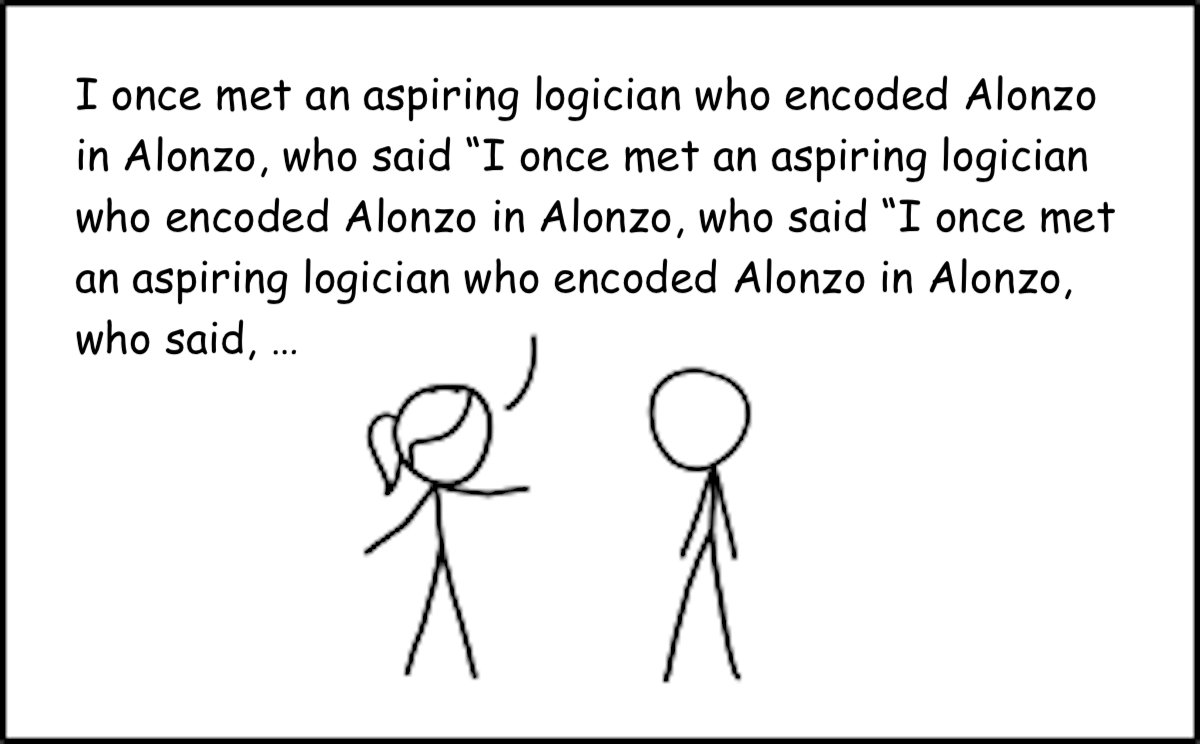
\includegraphics[width=10cm]{Alonzo.png}
\end{frame}


% \section{Free \& Bound Variables}
% \begin{frame}
% \frametitle{Sample frame title}
% This is some text in the first frame. This is some text in the first frame. This is some text in the first frame.
% \end{frame}


% \section{Substitutions}
% \begin{frame}
% \frametitle{Sample frame title}
% This is some text in the first frame. This is some text in the first frame. This is some text in the first frame.
% \end{frame}

\begin{frame}{References}
    \bibliographystyle{unsrtnat}
    \bibliography{main}
\end{frame}

\section{Appendix}
\begin{frame}{Appendix}
$\mName{INJ2} \text{ stands for }
\cFunAbs{f}{\cFunTyBX{\alpha}{\beta}{\gamma}}{\cInj{\cDefDesX{g}{\cFunTyX{\alpha \times \beta}{\gamma}}{\cForallBX{a}{\alpha}{b}{\beta}{\cQuasiEq{\cFunAppX{g}{(a,b)}}{\cFunAppBX{f}{a}{b}}}}}}
$
\end{frame}

\end{document}